\documentclass[12pt,a4paper]{article}
\usepackage[a4paper, margin=0.8in, headheight=14pt]{geometry}
\usepackage{fontspec}
\usepackage{unicode-math}
\setmainfont{TeX Gyre Pagella}
\setmonofont[Scale=0.88]{TeX Gyre Cursor}
\setmathfont{Latin Modern Math}
\usepackage{xcolor}
\usepackage{colortbl}
\usepackage{titlesec}
\usepackage{enumitem}
\usepackage{tabularx}
\usepackage{booktabs}
\usepackage{array}
\usepackage{amsmath}
\usepackage{tikz}
\usetikzlibrary{shapes.geometric, arrows.meta, positioning, calc, fit}
\usepackage{tcolorbox}
\tcbuselibrary{skins, breakable}
\usepackage{hyperref}
\usepackage{fancyhdr}
\usepackage{graphicx}
\usepackage{microtype}
\hyphenpenalty=10000
\exhyphenpenalty=10000
\sloppy
\usepackage{caption}
\usepackage{setspace}
\usepackage{multirow}
\usepackage{tocloft}
\newcommand{\Q}[1]{\textbf{#1}\par\noindent\ignorespaces}
\definecolor{myred}{RGB}{196,30,58}
\definecolor{mydark}{RGB}{30,30,50}
\definecolor{mygreen}{RGB}{14,120,80}
\definecolor{myteal}{RGB}{0,130,140}
\definecolor{myamber}{RGB}{180,100,0}
\definecolor{mypurple}{RGB}{100,30,160}
\definecolor{mygray}{RGB}{246,247,249}
\definecolor{mgframe}{RGB}{180,185,200}
\definecolor{watermark}{RGB}{145,150,170}
\definecolor{hdrred}{RGB}{250,232,235}
\definecolor{hdrgreen}{RGB}{220,244,233}
\definecolor{hdrteal}{RGB}{220,242,244}
\definecolor{hdramber}{RGB}{253,242,215}
\definecolor{hdrpurple}{RGB}{238,228,255}
\definecolor{hdrgray}{RGB}{238,240,245}
\definecolor{rowalt}{RGB}{250,251,253}
\titleformat{\section}{\large\bfseries\color{myred}}{\thesection.}{0.5em}{}
  [\vspace{1pt}{\color{myred}\rule{\linewidth}{0.8pt}}]
\titleformat{\subsection}{\normalsize\bfseries\color{myteal}}{\thesubsection}{0.5em}{}
\titlespacing*{\section}{0pt}{18pt}{7pt}
\titlespacing*{\subsection}{0pt}{11pt}{4pt}
\setlength{\parindent}{0pt}
\setlength{\parskip}{4pt}
\renewcommand{\cfttoctitlefont}{\large\bfseries\color{myred}}
\renewcommand{\cftaftertoctitle}{\par\noindent{\color{myred}\rule{\linewidth}{0.8pt}}}
\setlength{\cftbeforetoctitleskip}{0pt}
\setlength{\cftaftertoctitleskip}{6pt}
\renewcommand{\cftsecfont}{\normalsize\bfseries\color{mydark}}
\renewcommand{\cftsecpagefont}{\normalsize\bfseries\color{mydark}}
\renewcommand{\cftsecleader}{\cftdotfill{\cftdotsep}}
\setlength{\cftbeforesecskip}{7pt}
\renewcommand{\cftsubsecfont}{\small\color{mydark}}
\renewcommand{\cftsubsecpagefont}{\small\color{mydark}}
\setlength{\cftbeforesubsecskip}{3pt}
\setlength{\cftsubsecindent}{1.4em}
\renewcommand{\arraystretch}{1.45}
\setlength{\tabcolsep}{6pt}
\arrayrulecolor{mydark}
\newcolumntype{B}[1]{>{\small\bfseries\raggedright\arraybackslash}m{#1}}
\renewcommand{\tabularxcolumn}[1]{m{#1}}
\pagestyle{fancy}\fancyhf{}
\fancyhead[L]{\small\color{myred}\textbf{EC601}\;\color{mydark}--- Control System}
\fancyhead[R]{\small\color{myteal}\textbf{Module 6 Notes}}
\fancyfoot[C]{\small\color{mydark}\thepage}
\fancyfoot[R]{\small\color{watermark}\textit{\copyright\ Biraj}}
\renewcommand{\headrulewidth}{0.5pt}
\renewcommand{\footrulewidth}{0.3pt}
\hypersetup{colorlinks=true,linkcolor=myteal,urlcolor=myteal,
  pdfauthor={Biraj Sarkar},pdftitle={EC601 --- Module 6 Notes}}
\tcbset{
  tikzbox/.style={colback=mygray,colframe=mgframe,boxrule=0.6pt,arc=4pt,
    left=8pt,right=8pt,top=6pt,bottom=6pt,colbacktitle=mgframe,coltitle=mydark,fonttitle=\small\bfseries},
  defbox/.style={colback=hdrgreen,colframe=mygreen,boxrule=0.8pt,arc=4pt,
    left=9pt,right=9pt,top=6pt,bottom=6pt,colbacktitle=mygreen,coltitle=white,fonttitle=\small\bfseries},
  formulabox/.style={colback=hdrteal,colframe=myteal,boxrule=0.8pt,arc=4pt,
    left=9pt,right=9pt,top=7pt,bottom=7pt,colbacktitle=myteal,coltitle=white,fonttitle=\small\bfseries},
  examplebox/.style={colback=hdramber,colframe=myamber,boxrule=0.8pt,arc=4pt,
    left=9pt,right=9pt,top=6pt,bottom=6pt,colbacktitle=myamber,coltitle=white,fonttitle=\small\bfseries},
  masonbox/.style={colback=hdrpurple,colframe=mypurple,boxrule=0.8pt,arc=4pt,
    left=9pt,right=9pt,top=6pt,bottom=6pt,colbacktitle=mypurple,coltitle=white,fonttitle=\small\bfseries},
  exambox/.style={colback=hdrpurple,colframe=mypurple,boxrule=1pt,arc=5pt,
    left=10pt,right=10pt,top=8pt,bottom=8pt,colbacktitle=mypurple,coltitle=white,fonttitle=\bfseries, breakable, title after break={\textbf{Frequently Asked / Viva Questions (contd.)}}}
}
% Allow all boxes to break across pages
\tcbset{breakable}
\tikzset{
  block/.style={rectangle,draw=myteal,fill=hdrteal,text width=2.6cm,align=center,
    minimum height=0.95cm,font=\small,rounded corners=3pt,line width=0.7pt},
  wblock/.style={rectangle,draw=myteal,fill=hdrteal,text width=3.6cm,align=center,
    minimum height=0.95cm,font=\small,rounded corners=3pt,line width=0.7pt},
  redblock/.style={rectangle,draw=myred,fill=hdrred,text width=2.4cm,align=center,
    minimum height=0.95cm,font=\small,rounded corners=3pt,line width=0.7pt},
  sumjunc/.style={circle,draw=myamber,fill=hdramber,minimum size=0.62cm,font=\small,line width=0.8pt},
  arrow/.style={-Stealth,thick,color=mydark},
  redarrow/.style={-Stealth,thick,color=myred},
  line/.style={thick,color=mydark},
  axis/.style={-Stealth,thin,color=mydark}
}

\begin{document}
\begin{center}
  {\LARGE\bfseries\color{myred} EC601 --- Control System}\\[5pt]
  {\normalsize\color{mydark} Semester VI \quad$\bullet$\quad 3L:0T:0P \quad$\bullet$\quad 3 Credits}\\[3pt]
  {\normalsize\color{myteal}\textbf{Module 6 Exam Notes}}\\[3pt]
  {\small\color{mydark} CGEC \;$|$\; B.Tech ECE (2023--27) \;$|$\; \textit{Biraj Sarkar}}
\end{center}
\vspace{2pt}\noindent{\color{myred}\rule{\linewidth}{1.5pt}}\vspace{2pt}
\hypersetup{linkcolor=mydark}
\tableofcontents
\hypersetup{linkcolor=myteal}\newpage

%═══════════════════════════════════════════════════════════════════════════════
\section{Nonlinear Control Systems --- Basic Concepts}
%═══════════════════════════════════════════════════════════════════════════════

Real-world control systems are inherently nonlinear. Linear analysis (transfer functions, Bode plots, root locus) applies only when the system is linearised around an operating point. When nonlinearities are significant, dedicated nonlinear analysis methods are required.

\begin{tcolorbox}[defbox]
\textbf{Nonlinear System:} A system that does not satisfy the principle of superposition (additivity + homogeneity). Its behaviour depends on the \textit{magnitude} and \textit{nature} of the input, not just its frequency.\\[4pt]
\textbf{Key difference from linear systems:} Frequency of output may differ from input; multiple equilibrium points possible; limit cycles can exist; stability depends on initial conditions.
\end{tcolorbox}

\subsection{Common Nonlinearities in Control Systems}

\begin{tabularx}{\linewidth}{|B{3.0cm}|X|>{\centering\arraybackslash}X|}
\hline
\multicolumn{1}{|>{\centering\arraybackslash}p{3.0cm}|}{\textbf{\color{myteal}Nonlinearity}} &
\multicolumn{1}{>{\centering\arraybackslash}X|}{\textbf{\color{myteal}Description}} &
\textbf{\color{myteal}Example} \\
\hline
Saturation & Output limited to a maximum value regardless of input magnitude & Amplifier, actuator \\
\hline
Dead Zone & No output for small inputs below a threshold & Gear backlash, friction \\
\hline
Backlash & Hysteresis in mechanical coupling; output lags input reversal & Gear trains \\
\hline
Relay (On-Off) & Output switches between two fixed values & Thermostat, bang-bang control \\
\hline
Coulomb Friction & Constant opposing force independent of velocity & Sliding surfaces \\
\hline
Hysteresis & Output depends on history of input & Magnetic materials \\
\hline
\end{tabularx}

\begin{tcolorbox}[tikzbox, title={Common Nonlinearity Characteristics}]
\centering
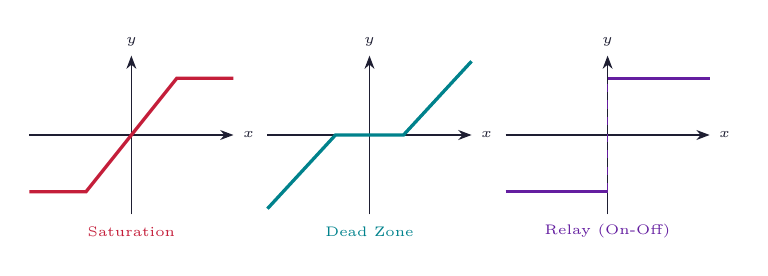
\begin{tikzpicture}[scale=0.72]
  % Saturation
  \begin{scope}[xshift=0cm]
    \draw[axis] (-1.8,0)--(1.8,0) node[right,font=\tiny]{$x$};
    \draw[axis] (0,-1.4)--(0,1.4) node[above,font=\tiny]{$y$};
    \draw[color=myred,line width=1.2pt] (-1.8,-1)--(-0.8,-1)--( 0.8,1)--(1.8,1);
    \node[font=\tiny,color=myred] at (0,-1.7) {Saturation};
  \end{scope}
  % Dead Zone
  \begin{scope}[xshift=4.2cm]
    \draw[axis] (-1.8,0)--(1.8,0) node[right,font=\tiny]{$x$};
    \draw[axis] (0,-1.4)--(0,1.4) node[above,font=\tiny]{$y$};
    \draw[color=myteal,line width=1.2pt] (-1.8,-1.3)--(-0.6,0)--(0.6,0)--(1.8,1.3);
    \node[font=\tiny,color=myteal] at (0,-1.7) {Dead Zone};
  \end{scope}
  % Relay
  \begin{scope}[xshift=8.4cm]
    \draw[axis] (-1.8,0)--(1.8,0) node[right,font=\tiny]{$x$};
    \draw[axis] (0,-1.4)--(0,1.4) node[above,font=\tiny]{$y$};
    \draw[color=mypurple,line width=1.2pt] (-1.8,-1)--(0,-1);
    \draw[color=mypurple,line width=1.2pt] (0,1)--(1.8,1);
    \draw[dashed,color=mypurple,thin] (0,-1)--(0,1);
    \node[font=\tiny,color=mypurple] at (0,-1.7) {Relay (On-Off)};
  \end{scope}
\end{tikzpicture}
\end{tcolorbox}

\subsection{Analysis Methods for Nonlinear Systems}

\begin{itemize}[leftmargin=*, itemsep=3pt]
  \item \textbf{Phase plane analysis:} Graphical method for 2nd order systems; plots $\dot{x}$ vs $x$.
  \item \textbf{Describing function method:} Frequency-domain approximation for nonlinear elements.
  \item \textbf{Lyapunov's method:} Energy-based stability analysis without solving the equations.
  \item \textbf{Linearisation:} Valid only near an operating point; uses Taylor series expansion.
\end{itemize}

%═══════════════════════════════════════════════════════════════════════════════
\section{Describing Function Method}
%═══════════════════════════════════════════════════════════════════════════════

\begin{tcolorbox}[defbox]
\textbf{Describing Function (DF):} An approximate frequency-domain representation of a nonlinear element. It is defined as the ratio of the \textit{fundamental harmonic component} of the output to the sinusoidal input, assuming the input is a pure sinusoid $x(t) = A\sin(\omega t)$.
$$N(A) = \frac{B_1 + jA_1}{A}$$
where $A_1$ and $B_1$ are the cosine and sine coefficients of the fundamental harmonic of the output.
\end{tcolorbox}

\subsection{Assumptions of the Describing Function Method}

\begin{enumerate}[label=\textbf{\arabic*.}, leftmargin=*, itemsep=3pt]
  \item The nonlinear element is \textbf{single-valued} (no memory/hysteresis) or has known hysteresis.
  \item The input to the nonlinear element is a \textbf{pure sinusoid}: $x(t) = A\sin(\omega t)$.
  \item The linear part of the system has \textbf{sufficient low-pass filtering} so that higher harmonics of the output are attenuated --- only the fundamental harmonic reaches the nonlinear element.
  \item The nonlinear element is \textbf{odd-symmetric}: $f(-x) = -f(x)$ (no even harmonics).
\end{enumerate}

\subsection{Describing Functions of Common Nonlinearities}

{\renewcommand{\arraystretch}{1.9}%
\begin{tabularx}{\linewidth}{|B{2.8cm}|>{\centering\arraybackslash}X|>{\raggedright\arraybackslash}X|}
\hline
\multicolumn{1}{|>{\centering\arraybackslash}m{2.8cm}|}{\textbf{\color{myteal}Nonlinearity}} &
\textbf{\color{myteal}Describing Function $N(A)$} &
\textbf{\color{myteal}Notes} \\
\hline
Ideal Relay & $\displaystyle\frac{4M}{\pi A}$ & $M$ = relay output level; real, decreases with $A$ \\[6pt]
\hline
Saturation & $\displaystyle\frac{2K}{\pi}\!\left[\sin^{-1}\!\!\left(\frac{D}{A}\right)+\frac{D}{A}\sqrt{1-\left(\frac{D}{A}\right)^{\!2}}\,\right]$ & $K$ = slope, $D$ = saturation level; valid for $A>D$ \\[6pt]
\hline
Dead Zone & \multicolumn{2}{>{\raggedright\arraybackslash}p{\dimexpr\linewidth-2.8cm-4\tabcolsep-3\arrayrulewidth}|}{%
  $\displaystyle K\!\left[1 - \frac{2}{\pi}\sin^{-1}\!\!\left(\frac{\Delta}{A}\right) - \frac{2\Delta}{\pi A}\sqrt{1-\left(\frac{\Delta}{A}\right)^{\!2}}\,\right]$
  \quad {\small($\Delta$ = dead zone half-width; valid for $A>\Delta$)}} \\[6pt]
\hline
Backlash & Complex (has imaginary part) & Phase lag introduced; $N(A)$ is complex \\
\hline
\end{tabularx}}

\subsection{Limit Cycle Prediction Using Describing Function}

The describing function method is primarily used to predict \textbf{limit cycles} --- sustained oscillations in nonlinear systems.

\begin{tcolorbox}[formulabox, title={Limit Cycle Condition}]
For a nonlinear system with nonlinear element $N(A)$ in the forward path and linear element $G(j\omega)$ in the loop, a limit cycle exists when:
$$G(j\omega)\cdot N(A) = -1 \quad \Rightarrow \quad G(j\omega) = -\frac{1}{N(A)}$$
\textbf{Graphical method:} Plot $G(j\omega)$ (Nyquist plot) and $-1/N(A)$ (negative inverse DF locus) on the same complex plane. Their \textbf{intersection} gives the limit cycle amplitude $A^*$ and frequency $\omega^*$.
\end{tcolorbox}

\begin{tcolorbox}[tikzbox, title={Limit Cycle Prediction --- Graphical Method}]
\centering
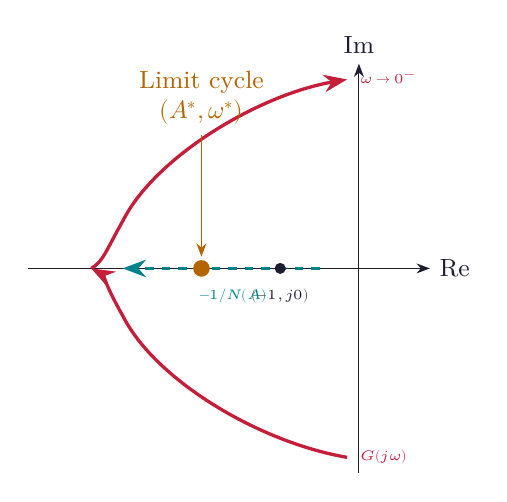
\begin{tikzpicture}[scale=1.0]
  % ── Axes ──────────────────────────────────────────────────────────────────
  \draw[-Stealth, thin, color=mydark] (-4.2,0)--(0.9,0) node[right,font=\small]{Re};
  \draw[-Stealth, thin, color=mydark] (0,-2.6)--(0,2.6) node[above,font=\small]{Im};

  % ── Nyquist plot of G(jω) — smooth Type-1 second order shape ─────────────
  % Lower half (omega: 0+ → infinity): starts at -j*infty (approx -2.4), sweeps left, ends near origin
  \draw[color=myred, line width=1.2pt, -Stealth]
    (-0.15,-2.4) .. controls (-1.3,-2.2) and (-2.6,-1.4) .. (-3.0,-0.6)
                 .. controls (-3.2,-0.25) and (-3.25,-0.08) .. (-3.4,0);
  % Upper half (mirror)
  \draw[color=myred, line width=1.2pt, -Stealth]
    (-3.4,0)     .. controls (-3.25,0.08) and (-3.2,0.25) .. (-3.0,0.6)
                 .. controls (-2.6,1.4) and (-1.3,2.2) .. (-0.15,2.4);

  % ── -1/N(A) locus (along negative real axis) ─────────────────────────────
  \draw[color=myteal, line width=1.2pt, dashed, -Stealth]
    (-0.5,0) -- (-3.0,0);

  % ── Critical (-1, j0) point ──────────────────────────────────────────────
  \fill[mydark] (-1,0) circle (2pt);
  \node[below=4pt, font=\tiny, color=mydark] at (-1,0) {$(-1, j0)$};

  % ── Limit cycle intersection ─────────────────────────────────────────────
  \fill[myamber] (-2.0,0) circle (3pt);
  % Annotation arrow + label well above the curve
  \draw[-Stealth, thin, color=myamber] (-2.0,1.7) -- (-2.0,0.15);
  \node[above, font=\small, color=myamber, align=center] at (-2.0,1.7)
    {Limit cycle\\$(A^*, \omega^*)$};

  % ── Curve labels (placed away from the action) ───────────────────────────
  \node[right, font=\tiny, color=myred] at (-0.1,-2.4) {$G(j\omega)$};
  \node[right, font=\tiny, color=myred] at (-0.1, 2.4) {$\omega \to 0^-$};
  \node[font=\tiny, color=myteal] at (-1.6,-0.35) {$-1/N(A)$};
\end{tikzpicture}
\end{tcolorbox}

\begin{tcolorbox}[exambox, title={Exam Tips --- Describing Function}]
\begin{itemize}[leftmargin=*, itemsep=3pt, topsep=0pt]
  \item DF is an \textbf{approximation} --- valid only when higher harmonics are filtered by the linear part.
  \item DF of ideal relay: $N(A) = 4M/(\pi A)$ --- purely real, decreases as $A$ increases.
  \item \textbf{Limit cycle} exists at intersection of $G(j\omega)$ and $-1/N(A)$ loci.
  \item If $-1/N(A)$ locus does \textbf{not intersect} $G(j\omega)$: no limit cycle predicted.
  \item \textbf{Stability of limit cycle:} If increasing $A$ moves $-1/N(A)$ outside $G(j\omega)$, the limit cycle is stable.
  \item DF method cannot detect \textbf{subharmonic oscillations} or \textbf{chaotic behaviour}.
\end{itemize}
\end{tcolorbox}

%═══════════════════════════════════════════════════════════════════════════════
\section{Introduction to Optimal Control}
%═══════════════════════════════════════════════════════════════════════════════

\begin{tcolorbox}[defbox]
\textbf{Optimal Control:} A control strategy that minimises (or maximises) a specified \textbf{performance index} (cost function) $J$ while satisfying the system dynamics and constraints. It provides the \textit{best possible} control in a mathematically defined sense.\\[4pt]
\textbf{Performance Index (Cost Function):} A scalar measure of system performance. Common form:
$$J = \int_0^{t_f} L(\mathbf{x}(t),\, \mathbf{u}(t),\, t)\, dt + \phi(\mathbf{x}(t_f))$$
where $L$ is the running cost and $\phi$ is the terminal cost.
\end{tcolorbox}

\subsection{Quadratic Performance Index (LQR)}

The most widely used performance index for linear systems is the \textbf{quadratic} form:

\begin{tcolorbox}[formulabox, title={Quadratic Performance Index}]
$$J = \int_0^{\infty} \left[\mathbf{x}^T(t)\,\mathbf{Q}\,\mathbf{x}(t) + \mathbf{u}^T(t)\,\mathbf{R}\,\mathbf{u}(t)\right] dt$$
where:
\begin{itemize}[leftmargin=*, itemsep=2pt, topsep=2pt]
  \item $\mathbf{Q}$ ($n\times n$, positive semi-definite) --- penalises state deviation from zero
  \item $\mathbf{R}$ ($r\times r$, positive definite) --- penalises control effort
  \item Large $\mathbf{Q}$: fast state regulation (aggressive control)
  \item Large $\mathbf{R}$: small control effort (gentle control)
\end{itemize}
The optimal control law is: $\mathbf{u}^*(t) = -\mathbf{R}^{-1}\mathbf{B}^T\mathbf{P}\,\mathbf{x}(t) = -\mathbf{K}\,\mathbf{x}(t)$\\
where $\mathbf{P}$ satisfies the \textbf{Algebraic Riccati Equation (ARE):}
$$\mathbf{A}^T\mathbf{P} + \mathbf{P}\mathbf{A} - \mathbf{P}\mathbf{B}\mathbf{R}^{-1}\mathbf{B}^T\mathbf{P} + \mathbf{Q} = \mathbf{0}$$
\end{tcolorbox}

\subsection{Regulator Problem}

\begin{tcolorbox}[defbox]
\textbf{Regulator Problem:} Drive the state $\mathbf{x}(t)$ to \textbf{zero} (or maintain it at zero) in the presence of disturbances, starting from a non-zero initial condition $\mathbf{x}(0) \neq \mathbf{0}$.\\[4pt]
\textbf{Goal:} $\mathbf{x}(t) \to \mathbf{0}$ as $t \to \infty$, while minimising the cost $J$.\\[4pt]
\textbf{Reference:} $\mathbf{r}(t) = \mathbf{0}$ (zero reference). The system must reject disturbances and return to equilibrium.\\[4pt]
\textbf{Example:} Stabilising an inverted pendulum at the upright position.
\end{tcolorbox}

\begin{tcolorbox}[tikzbox, title={Regulator Problem Block Diagram}]
\centering
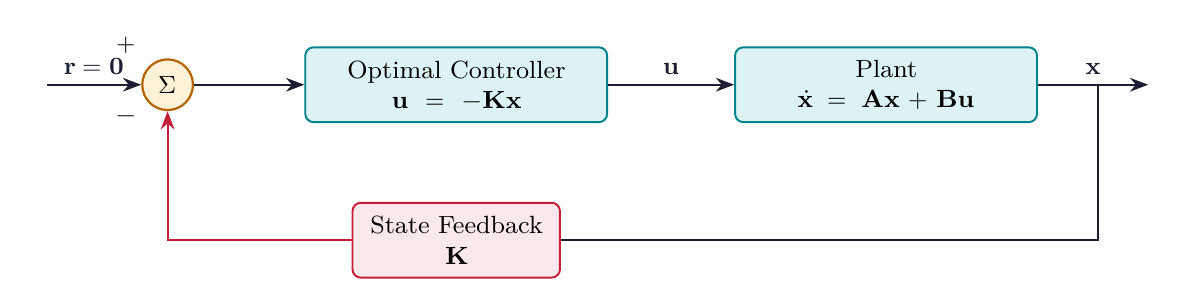
\begin{tikzpicture}[node distance=0.5cm and 1.5cm]
  \node[sumjunc] (sum) {$\Sigma$};
  \node[wblock, right=1.4cm of sum] (ctrl) {Optimal Controller\\$\mathbf{u}=-\mathbf{K}\mathbf{x}$};
  \node[wblock, right=1.6cm of ctrl] (plant) {Plant\\$\dot{\mathbf{x}}=\mathbf{A}\mathbf{x}+\mathbf{B}\mathbf{u}$};
  \node[left=1.2cm of sum] (ref) {};
  \node[right=1.4cm of plant] (out) {};
  \node[redblock, below=1.0cm of ctrl] (fb) {State Feedback\\$\mathbf{K}$};
  \draw[arrow] (ref) -- node[above]{\small $\mathbf{r}=\mathbf{0}$} (sum);
  \draw[arrow] (sum) -- (ctrl);
  \draw[arrow] (ctrl) -- node[above]{\small $\mathbf{u}$} (plant);
  \draw[arrow] (plant) -- node[above]{\small $\mathbf{x}$} (out);
  \coordinate (xtap) at ($(plant.east)!0.5!(out)$);
  \draw[line] (xtap) |- (fb.east);
  \draw[redarrow] (fb.west) -| (sum.south);
  \node[above left=1pt and 1pt of sum]{\small $+$};
  \node[below left=1pt and 1pt of sum]{\small $-$};
\end{tikzpicture}
\end{tcolorbox}

\subsection{Output Regulator Problem}

\begin{tcolorbox}[defbox]
\textbf{Output Regulator Problem:} A variant of the regulator problem where the \textbf{output} $\mathbf{y}(t)$ (not the full state) is driven to zero. The performance index penalises the output rather than the full state:
$$J = \int_0^{\infty} \left[\mathbf{y}^T\mathbf{Q}_y\mathbf{y} + \mathbf{u}^T\mathbf{R}\mathbf{u}\right] dt = \int_0^{\infty} \left[\mathbf{x}^T\mathbf{C}^T\mathbf{Q}_y\mathbf{C}\,\mathbf{x} + \mathbf{u}^T\mathbf{R}\mathbf{u}\right] dt$$
This is equivalent to the state regulator with $\mathbf{Q} = \mathbf{C}^T\mathbf{Q}_y\mathbf{C}$.\\[4pt]
\textbf{Use case:} When only the output (not all states) needs to be regulated, and full state measurement is unavailable.
\end{tcolorbox}

\subsection{Tracking Problem}

\begin{tcolorbox}[defbox]
\textbf{Tracking Problem:} The output $\mathbf{y}(t)$ must \textbf{follow} (track) a desired reference trajectory $\mathbf{r}(t) \neq \mathbf{0}$. The error $\mathbf{e}(t) = \mathbf{r}(t) - \mathbf{y}(t)$ must be minimised.\\[4pt]
\textbf{Performance index:}
$$J = \int_0^{t_f} \left[\mathbf{e}^T(t)\,\mathbf{Q}\,\mathbf{e}(t) + \mathbf{u}^T(t)\,\mathbf{R}\,\mathbf{u}(t)\right] dt$$
\textbf{Example:} Robot arm tracking a desired trajectory; missile tracking a moving target; CNC machine following a path.
\end{tcolorbox}

\begin{tabularx}{\linewidth}{|B{2.8cm}|>{\centering\arraybackslash}X|>{\centering\arraybackslash}X|>{\centering\arraybackslash}X|}
\hline
\multicolumn{1}{|>{\centering\arraybackslash}p{2.8cm}|}{\textbf{Problem}} &
\textbf{\color{myamber}Reference} & \textbf{\color{mygreen}Goal} & \textbf{\color{myteal}Example} \\
\hline
Regulator & $\mathbf{r}=\mathbf{0}$ & $\mathbf{x}(t)\to\mathbf{0}$ & Stabilise inverted pendulum \\
\hline
Output Regulator & $\mathbf{r}=\mathbf{0}$ & $\mathbf{y}(t)\to\mathbf{0}$ & Regulate output only \\
\hline
Tracking & $\mathbf{r}(t)\neq\mathbf{0}$ & $\mathbf{y}(t)\to\mathbf{r}(t)$ & Robot arm trajectory \\
\hline
\end{tabularx}

\begin{tcolorbox}[exambox, title={Exam Tips --- Optimal Control}]
\begin{itemize}[leftmargin=*, itemsep=3pt, topsep=0pt]
  \item \textbf{LQR} = Linear Quadratic Regulator; optimal for linear systems with quadratic cost.
  \item \textbf{$\mathbf{Q}$ large} $\Rightarrow$ fast state regulation; \textbf{$\mathbf{R}$ large} $\Rightarrow$ small control effort.
  \item Optimal gain: $\mathbf{K} = \mathbf{R}^{-1}\mathbf{B}^T\mathbf{P}$ where $\mathbf{P}$ solves the Algebraic Riccati Equation.
  \item \textbf{Regulator:} zero reference, drive state to zero. \textbf{Tracking:} non-zero reference, follow trajectory.
  \item \textbf{Output regulator:} only output penalised; equivalent to state regulator with $\mathbf{Q}=\mathbf{C}^T\mathbf{Q}_y\mathbf{C}$.
  \item Optimal control requires the system to be \textbf{controllable} (otherwise $J$ cannot be minimised).
\end{itemize}
\end{tcolorbox}

%═══════════════════════════════════════════════════════════════════════════════
\newpage
\begin{center}
  {\large\bfseries\color{myred} Quick Revision --- Module 6}\\[3pt]
  {\small\color{mydark} Nonlinear Systems \& Optimal Control $|$ EC601}
\end{center}
\noindent{\color{myred}\rule{\linewidth}{1.2pt}}\vspace{4pt}

\begin{tcolorbox}[formulabox, title={\textbf{Key Formulas at a Glance}}]
\begin{tabularx}{\linewidth}{B{5.0cm} X}
DF of ideal relay           & $N(A) = 4M/(\pi A)$ \\[2pt]
Limit cycle condition       & $G(j\omega) = -1/N(A)$ \\[2pt]
Quadratic cost function     & $J = \int_0^\infty (\mathbf{x}^T\mathbf{Q}\mathbf{x} + \mathbf{u}^T\mathbf{R}\mathbf{u})\,dt$ \\[2pt]
Optimal control law (LQR)   & $\mathbf{u}^* = -\mathbf{K}\mathbf{x} = -\mathbf{R}^{-1}\mathbf{B}^T\mathbf{P}\mathbf{x}$ \\[2pt]
Algebraic Riccati Eq.       & $\mathbf{A}^T\mathbf{P}+\mathbf{P}\mathbf{A}-\mathbf{P}\mathbf{B}\mathbf{R}^{-1}\mathbf{B}^T\mathbf{P}+\mathbf{Q}=\mathbf{0}$ \\[2pt]
Output regulator $\mathbf{Q}$ & $\mathbf{Q} = \mathbf{C}^T\mathbf{Q}_y\mathbf{C}$ \\[2pt]
Tracking error              & $\mathbf{e}(t) = \mathbf{r}(t) - \mathbf{y}(t)$
\end{tabularx}
\end{tcolorbox}

\vspace{5pt}

\begin{tcolorbox}[defbox, title={\textbf{One-Line Definitions}}]
\begin{itemize}[leftmargin=*, itemsep=3pt, topsep=0pt]
  \item \textbf{Nonlinear system:} Does not satisfy superposition; output depends on input magnitude.
  \item \textbf{Saturation:} Output limited to a maximum value regardless of input.
  \item \textbf{Dead zone:} No output for inputs below a threshold.
  \item \textbf{Limit cycle:} Sustained periodic oscillation in a nonlinear system.
  \item \textbf{Describing Function:} Ratio of fundamental harmonic output to sinusoidal input; $N(A)$.
  \item \textbf{Optimal control:} Minimises a performance index $J$ while satisfying system dynamics.
  \item \textbf{LQR:} Linear Quadratic Regulator; optimal state feedback for linear systems.
  \item \textbf{Regulator problem:} Drive state to zero from non-zero initial condition.
  \item \textbf{Output regulator:} Drive output (not full state) to zero.
  \item \textbf{Tracking problem:} Output must follow a non-zero reference trajectory.
  \item \textbf{Riccati equation:} Matrix equation whose solution $\mathbf{P}$ gives the optimal gain $\mathbf{K}$.
\end{itemize}
\end{tcolorbox}

\vspace{5pt}

\begin{tcolorbox}[exambox, title={\textbf{Frequently Asked / Viva Questions}}]
\begin{enumerate}[topsep=0pt, label=\textbf{Q\arabic*.}, itemsep=5pt]
  \item \Q{What is a nonlinear system?}
    A system that does not satisfy superposition (additivity + homogeneity). Its behaviour depends on input magnitude and initial conditions.
  \item \Q{Name four common nonlinearities in control systems.}
    Saturation, dead zone, backlash, relay (on-off), Coulomb friction, hysteresis.
  \item \Q{What is the Describing Function?}
    An approximate frequency-domain representation of a nonlinear element. $N(A)$ = ratio of fundamental harmonic output to sinusoidal input amplitude $A$.
  \item \Q{What is the DF of an ideal relay?}
    $N(A) = 4M/(\pi A)$, where $M$ is the relay output level. It is purely real and decreases as $A$ increases.
  \item \Q{How is a limit cycle predicted using the DF method?}
    Plot $G(j\omega)$ (Nyquist) and $-1/N(A)$ on the same complex plane. Their intersection gives the limit cycle amplitude $A^*$ and frequency $\omega^*$.
  \item \Q{What are the assumptions of the DF method?}
    Sinusoidal input to nonlinear element; linear part has sufficient low-pass filtering; nonlinearity is odd-symmetric; single-valued (or known hysteresis).
  \item \Q{What is the optimal control problem?}
    Find the control $\mathbf{u}(t)$ that minimises a performance index $J$ subject to the system dynamics $\dot{\mathbf{x}}=\mathbf{A}\mathbf{x}+\mathbf{B}\mathbf{u}$.
  \item \Q{What is the LQR cost function?}
    $J = \int_0^\infty (\mathbf{x}^T\mathbf{Q}\mathbf{x} + \mathbf{u}^T\mathbf{R}\mathbf{u})\,dt$. $\mathbf{Q}$ penalises state deviation; $\mathbf{R}$ penalises control effort.
  \item \Q{What is the regulator problem?}
    Drive the state $\mathbf{x}(t)\to\mathbf{0}$ from a non-zero initial condition, with zero reference input, while minimising $J$.
  \item \Q{What is the difference between regulator and tracking?}
    Regulator: reference is zero, goal is to drive state/output to zero. Tracking: reference is non-zero, goal is to follow the reference trajectory.
  \item \Q{What is the Algebraic Riccati Equation?}
    $\mathbf{A}^T\mathbf{P}+\mathbf{P}\mathbf{A}-\mathbf{P}\mathbf{B}\mathbf{R}^{-1}\mathbf{B}^T\mathbf{P}+\mathbf{Q}=\mathbf{0}$. Its solution $\mathbf{P}$ gives the optimal gain $\mathbf{K}=\mathbf{R}^{-1}\mathbf{B}^T\mathbf{P}$.
\end{enumerate}
\end{tcolorbox}

\end{document}
